\documentclass[11pt,letterpaper]{article}

\usepackage[utf8]{inputenc}
\usepackage[T1]{fontenc}
\usepackage[spanish,es-noquoting]{babel}
\usepackage[margin=2.5cm]{geometry}
\usepackage{graphicx}
\usepackage{booktabs}
\usepackage{float}
\usepackage{caption}
\usepackage{amsmath}
\usepackage[hidelinks]{hyperref}

\graphicspath{{figuras/}}
\captionsetup{font=small,labelfont=bf}
\setlength{\parskip}{0.6em}
\setlength{\parindent}{0pt}

\title{\vspace{-1.5cm}\textbf{Proyecto 2. Análisis Exploratorio}\\[0.3em]
\large Reto 18: Hackeando el cuerpo humano\\
\normalsize HuBMAP + HPA --- Segmentación de unidades funcionales de tejido}

% TODO: reemplazar por los nombres completos y carnés reales de cada integrante
\author{Nombre Apellido --- 00000 \and Nombre Apellido --- 00000 \and Nombre Apellido --- 00000}
\date{Universidad del Valle de Guatemala\\
Facultad de Ingeniería --- Departamento de Ciencias de la Computación\\
CC3084 Data Science --- Semestre II, 2026\\[0.5em]
\today}

\begin{document}

\maketitle

\begin{abstract}
\noindent
Este informe presenta el análisis exploratorio del conjunto de datos de la competencia
\emph{HuBMAP - Hacking the Human Body}, cuyo objetivo es segmentar unidades funcionales de tejido
(FTU) en imágenes de cortes histológicos de cinco órganos humanos. Se analizaron las 351
observaciones del archivo \texttt{train.csv}, se construyó una variable derivada a partir de la
máscara codificada en \emph{run-length encoding} y se documentaron los hallazgos que condicionan
cualquier intento posterior de modelado. Los resultados principales son la ausencia total de
muestras HuBMAP en el conjunto de entrenamiento, la existencia de variables numéricas constantes,
un desbalance simultáneo en órgano, sexo y edad, una variable objetivo fuertemente desbalanceada a
nivel de píxel, y una correlación global entre edad y tamaño de FTU que se revela espuria al
controlar por órgano.
\end{abstract}

\tableofcontents
\newpage

%======================================================================
\section{Investigación del tema}
%======================================================================

HuBMAP (\emph{Human BioMolecular Atlas Program}) es un programa que busca mapear el cuerpo humano a
nivel de célula, es decir, construir un mapa detallado de cómo están organizados los tejidos sanos
en cada órgano. La competencia de Kaggle nace de ese programa y combina datos de HuBMAP con los del
Atlas de Proteínas Humanas (HPA). Lo que pide es encontrar y delimitar, dentro de fotografías de
tejido, las llamadas unidades funcionales de tejido o FTU.

Una FTU es un grupo pequeño de células organizadas alrededor de un vaso sanguíneo que en conjunto
cumplen una función específica dentro del órgano al que pertenecen. El reto incluye cinco órganos:
riñón, próstata, bazo, pulmón e intestino grueso. En cada uno la FTU se ve distinta porque cada
órgano tiene su propia estructura: en riñón corresponde a los glomérulos, en intestino grueso a las
criptas, en próstata a las unidades glandulares.

\subsection{Sobre el diagnóstico basado en imágenes}

Las imágenes provienen de cortes de tejido teñidos con PAS (\emph{Periodic Acid-Schiff}), una
tinción que reacciona con los carbohidratos del tejido y resalta membranas basales y estructuras
glandulares, de modo que puedan distinguirse al microscopio. Ese es el motivo del característico
tono rosado y morado de las muestras.

El patrón que un algoritmo debe reconocer no es una lesión ni una enfermedad, sino una estructura
anatómica normal: la organización espacial de células alrededor de un vaso. La dificultad
diagnóstica está en que esa organización cambia de forma, tamaño y contraste según el órgano, y en
que la apariencia del tejido depende también de cómo se preparó y escaneó la muestra.

Como los datos provienen de dos fuentes distintas, y cada una prepara y escanea las muestras a su
manera, un mismo órgano puede verse diferente según de dónde salió la imagen. Este punto es central:
la meta es que el modelo reconozca las FTU sin importar el órgano ni la fuente, y no que memorice
los casos que vio durante el entrenamiento.

%======================================================================
\section{Análisis del problema planteado y los datos}
%======================================================================

\subsection{Situación problemática}

Actualmente, identificar las unidades funcionales de tejido en una imagen de biopsia lo hacen
patólogos a mano, revisando la muestra al microscopio y marcando dónde están esas estructuras. El
procedimiento toma tiempo, depende de la experiencia de la persona que lo realiza y no es escalable
a miles de imágenes de distintos órganos.

A eso se suma un problema de consistencia: como las muestras pueden venir de laboratorios distintos
con procesos de preparación distintos, dos imágenes del mismo órgano no siempre se ven igual. Esto
complica todavía más hacer el trabajo de forma manual y reproducible, e introduce variabilidad entre
observadores que es difícil de cuantificar.

\subsection{Problema científico}

El problema se formula como una tarea de segmentación semántica: a partir de una imagen de tejido,
¿se puede entrenar un modelo que marque con precisión en qué zonas de la imagen se encuentran las
unidades funcionales de tejido, sin importar de qué órgano se trate ni de qué fuente provenga la
muestra?

La dificultad adicional es que el conjunto de datos solo contiene unos cuantos órganos y fuentes, de
manera que el modelo debe aprender un patrón que generalice en lugar de memorizar la apariencia
particular de cada órgano.

\subsection{Objetivos}

\textbf{Objetivo general.} Explorar y describir los datos de la competencia HuBMAP para entender
cómo están compuestas las imágenes de tejido y las variables que las acompañan, de forma que sirva
de base para plantear una futura solución al problema de segmentación de FTU.

\textbf{Objetivos específicos.}
\begin{enumerate}
  \item Describir las variables numéricas y categóricas del conjunto de datos (órgano, fuente,
        edad, sexo, grosor del tejido, dimensiones de imagen) y detectar diferencias entre grupos.
  \item Analizar cómo se relacionan órgano, fuente de datos, edad y sexo, para identificar qué tan
        variadas son las imágenes según esos factores.
  \item Cuantificar el área que ocupa la FTU dentro de cada imagen y comparar su distribución entre
        órganos, para dimensionar el desbalance de clases del problema de segmentación.
\end{enumerate}

%======================================================================
\section{Descripción de los datos y limpieza}
%======================================================================

\subsection{Origen y estructura}

Se trabajó únicamente con el archivo \texttt{train.csv}, que es el único que trae etiquetas
completas, ya que no se participó en la competencia como tal. El archivo tiene 351 filas y 10
columnas. Cada fila corresponde a una imagen de tejido con su información asociada.

\begin{table}[H]
\centering
\caption{Variables disponibles en \texttt{train.csv}}
\begin{tabular}{llp{7.6cm}}
\toprule
\textbf{Variable} & \textbf{Tipo} & \textbf{Descripción} \\
\midrule
\texttt{id}               & Identificador & Código de la imagen. Sin valor analítico propio. \\
\texttt{organ}            & Categórica    & Órgano de la muestra (5 niveles). \\
\texttt{data\_source}     & Categórica    & Fuente de la muestra (HuBMAP o HPA). \\
\texttt{img\_height}      & Numérica      & Alto de la imagen en píxeles. \\
\texttt{img\_width}       & Numérica      & Ancho de la imagen en píxeles. \\
\texttt{pixel\_size}      & Numérica      & Micrómetros representados por cada píxel. \\
\texttt{tissue\_thickness}& Numérica      & Grosor del corte de tejido. \\
\texttt{rle}              & Texto         & Máscara de la FTU codificada en run-length encoding. \\
\texttt{age}              & Numérica      & Edad del donante en años. \\
\texttt{sex}              & Categórica    & Sexo del donante. \\
\bottomrule
\end{tabular}
\end{table}

La columna \texttt{rle} merece una aclaración porque no es una variable convencional. El formato
\emph{run-length encoding} no almacena la máscara píxel por píxel, sino pares de números
(posición inicial, longitud) que indican tramos consecutivos de píxeles marcados. Guardar una
máscara de $3000 \times 3000$ como matriz sería inviable dentro de una celda de texto; el rle la
comprime a unos cuantos miles de caracteres.

\subsection{Limpieza y preprocesamiento}

No se encontraron valores nulos ni filas duplicadas en \texttt{train.csv}, de modo que no fue
necesario eliminar ni imputar ninguna observación. La única operación aplicada fue convertir
\texttt{organ}, \texttt{data\_source} y \texttt{sex} a tipo categórico, ya que pandas las cargaba
como texto plano y el tipo categórico las identifica correctamente como conjuntos cerrados de
valores.

La columna \texttt{rle} no se decodifica de forma completa para todo el conjunto, porque
reconstruir 351 máscaras de nueve millones de píxeles cada una es costoso y no aporta nada al
análisis tabular. La decodificación completa se reserva para la muestra de imágenes usada en la
sección visual.

%======================================================================
\section{Análisis exploratorio}
%======================================================================

\subsection{Variables y observaciones disponibles}

El conjunto tiene 351 observaciones, una por imagen de tejido, y 10 variables. Tres son categóricas
(\texttt{organ}, \texttt{data\_source}, \texttt{sex}), cinco son numéricas (\texttt{img\_height},
\texttt{img\_width}, \texttt{pixel\_size}, \texttt{tissue\_thickness}, \texttt{age}), una es un
identificador (\texttt{id}) y una es texto estructurado (\texttt{rle}). No hay valores faltantes en
ninguna de las 351 filas.

\subsection{Resumen de las variables numéricas}

\begin{table}[H]
\centering
\caption{Estadísticos descriptivos de las variables numéricas}
\begin{tabular}{lrrrrrr}
\toprule
& \textbf{media} & \textbf{desv.\ est.} & \textbf{mín} & \textbf{Q1} & \textbf{mediana} & \textbf{máx} \\
\midrule
\texttt{img\_height}       & 2978.4 & 91.0 & 2308 & 3000 & 3000 & 3070 \\
\texttt{img\_width}        & 2978.4 & 91.0 & 2308 & 3000 & 3000 & 3070 \\
\texttt{pixel\_size}       & 0.4    & 0.0  & 0.4  & 0.4  & 0.4  & 0.4  \\
\texttt{tissue\_thickness} & 4.0    & 0.0  & 4    & 4    & 4    & 4    \\
\texttt{age}               & 60.4   & 16.0 & 21   & 55   & 60   & 84   \\
\bottomrule
\end{tabular}
\end{table}

Casi todas las imágenes miden $3000 \times 3000$ píxeles: la mediana y el percentil 75 de
\texttt{img\_height} e \texttt{img\_width} caen exactamente en 3000, y el mínimo de 2308 indica que
existen algunas imágenes más pequeñas, aunque la variación es baja frente al tamaño típico
(desviación estándar de aproximadamente 91 píxeles). Además, en las 351 filas el alto y el ancho
coinciden siempre, es decir que todas las imágenes son cuadradas.

\texttt{pixel\_size} y \texttt{tissue\_thickness} no varían en absoluto: valen 0.4 y 4 en las 351
filas, con desviación estándar cero. En este archivo no aportan ninguna información para diferenciar
observaciones. La explicación aparece en la tabla de frecuencias de la sección siguiente:
\texttt{train.csv} solo contiene imágenes de origen HPA, que se escanean siempre con esos mismos
parámetros. En el conjunto de HuBMAP estos valores sí varían.

En cuanto a \texttt{age} hay dispersión considerable: el promedio es de 60 años, con donantes entre
21 y 84 años y una desviación estándar de 16 años, lo que indica que el conjunto cubre un rango
amplio de edades adultas.

\subsection{Tablas de frecuencia de las variables categóricas}

\begin{table}[H]
\centering
\caption{Distribución de las variables categóricas}
\begin{tabular}{llrr}
\toprule
\textbf{Variable} & \textbf{Nivel} & \textbf{Frecuencia} & \textbf{Proporción} \\
\midrule
\texttt{organ} & kidney         & 99 & 28.2\,\% \\
               & prostate       & 93 & 26.5\,\% \\
               & largeintestine & 58 & 16.5\,\% \\
               & spleen         & 53 & 15.1\,\% \\
               & lung           & 48 & 13.7\,\% \\
\midrule
\texttt{data\_source} & HPA    & 351 & 100.0\,\% \\
                      & HuBMAP &   0 &   0.0\,\% \\
\midrule
\texttt{sex} & Male   & 229 & 65.2\,\% \\
             & Female & 122 & 34.8\,\% \\
\bottomrule
\end{tabular}
\end{table}

En \texttt{organ}, riñón (99) y próstata (93) son los órganos con más observaciones, seguidos de
intestino grueso (58), bazo (53) y pulmón (48, el menos representado). No es un desbalance extremo,
pero conviene tenerlo en cuenta al comparar métricas entre órganos.

En \texttt{data\_source}, el 100\,\% de las filas provienen de HPA: no hay ninguna observación de
HuBMAP en \texttt{train.csv}. Este es un hallazgo importante. Aunque la competencia combina ambas
fuentes, el archivo con el que se trabaja solo contiene la parte pública de HPA, mientras que las
muestras de HuBMAP quedan en el conjunto de prueba oculto. En consecuencia, este análisis describe
solo esa porción de los datos y no el problema completo.

En \texttt{sex}, el 65.2\,\% de los donantes son hombres (229) y el 34.8\,\% mujeres (122). Este
desbalance se explica en parte por \texttt{prostate}, que por razones biológicas solo tiene donantes
hombres, como se revisa en el cruce de variables.

\subsection{Cruce de variables}

\begin{table}[H]
\centering
\caption{Tabla de contingencia entre órgano y sexo}
\begin{tabular}{lrrr}
\toprule
\textbf{Órgano} & \textbf{Female} & \textbf{Male} & \textbf{\% Male} \\
\midrule
kidney         & 37 & 62 & 62.6\,\% \\
prostate       &  0 & 93 & 100.0\,\% \\
largeintestine & 32 & 26 & 44.8\,\% \\
spleen         & 28 & 25 & 47.2\,\% \\
lung           & 25 & 23 & 47.9\,\% \\
\bottomrule
\end{tabular}
\end{table}

El cruce de \texttt{organ} con \texttt{sex} explica buena parte del desbalance de sexo:
\texttt{prostate} es 100\,\% masculino (93 de 93), lo cual es un patrón esperado por la biología del
órgano y no un error de datos. \texttt{kidney} también se inclina hacia hombres (63\,\%), mientras
que intestino grueso, pulmón y bazo están bastante más parejos (45 a 55\,\%). Como próstata es el
segundo órgano más frecuente, entre ese y riñón explican casi todo el desbalance general observado.

El cruce de \texttt{organ} con \texttt{age} muestra que \texttt{largeintestine} es un caso claramente
distinto: su edad mediana es de 83 años, muy por encima de los otros cuatro órganos, que rondan entre
53 y 60 años de mediana. Esto indica que \texttt{organ} y \texttt{age} no son independientes en este
conjunto. No parece un error, sino el resultado de cómo se repartieron los donantes por tipo de
muestra, pero es importante tenerlo presente: cualquier patrón que se observe en \texttt{age} puede
en realidad estar reflejando de qué órgano proviene la imagen.

\subsection{Correlaciones}

La matriz de correlación no muestra relaciones lineales relevantes entre las variables numéricas
originales. La correlación entre \texttt{age} e \texttt{img\_height} o \texttt{img\_width} es
prácticamente nula (0.04), y con \texttt{id} también (0.02, esperable porque \texttt{id} es solo un
identificador sin significado real). \texttt{img\_height} e \texttt{img\_width} correlacionan
perfectamente entre sí (1.0), lo cual tiene sentido porque todas las imágenes son cuadradas.

\texttt{pixel\_size} y \texttt{tissue\_thickness} aparecen como \texttt{NaN} en toda la matriz. Esto
no es un error de cálculo: al ser constantes, su desviación estándar es cero y el coeficiente de
Pearson queda indefinido porque implica una división entre cero. Dentro de las variables numéricas
originales no hay pares que valga la pena modelar juntos por una relación lineal; lo interesante del
conjunto está en las categóricas y en sus cruces.

\subsection{Outliers y valores faltantes}

En \texttt{age}, el método del rango intercuartílico marca 13 outliers (límites de 28 a 100 años),
todos con valor 21 años, el mínimo del conjunto. Sin embargo, como se vio en el cruce con
\texttt{organ}, la edad depende bastante del órgano: 21 años cae dentro del rango normal de pulmón y
bazo, así que estos outliers globales no son errores ni casos raros, sino donantes jóvenes que
resultan atípicos solo si se ignora a qué órgano pertenecen. No se eliminó ni transformó ninguna
observación; se documenta el hallazgo.

En \texttt{img\_height} el resultado es distinto. Como el 75\,\% de las imágenes miden exactamente
3000 px, el rango intercuartílico es cero y el método marca como outlier cualquier imagen que no
mida 3000 (25 de 351, concentradas en riñón y próstata). Aquí el método clásico no resulta útil
porque la variable no es continua en la práctica, sino casi binaria: 3000 o no 3000. La explicación
más probable es que esas imágenes sean recortes de tejido que no alcanzaron el tamaño estándar de
escaneo, no errores de carga, de modo que tampoco se descartan.

Sobre valores faltantes, \texttt{train.csv} no presenta ningún valor nulo en sus 351 filas, por lo
que no fue necesaria ninguna decisión de imputación o eliminación.

\subsection{Variable derivada: área de la FTU}

Las variables tabulares originales dicen poco sobre el problema real. La información que de verdad
importa está dentro de la columna \texttt{rle}, porque es la que describe lo que el modelo debe
predecir. Por eso se construyó una variable derivada.

Aprovechando que el formato rle almacena pares (inicio, longitud), basta con sumar las longitudes
para obtener la cantidad de píxeles marcados, sin necesidad de reconstruir la máscara completa. A
partir de ahí se define:

\begin{equation*}
\texttt{mask\_frac} = \frac{\text{píxeles marcados como FTU}}
                           {\texttt{img\_height} \times \texttt{img\_width}}
\end{equation*}

es decir, la proporción de la imagen ocupada por la unidad funcional de tejido.

\begin{table}[H]
\centering
\caption{Proporción de la imagen ocupada por la FTU, por órgano}
\begin{tabular}{lrrrrr}
\toprule
\textbf{Órgano} & \textbf{n} & \textbf{media} & \textbf{mediana} & \textbf{mín} & \textbf{máx} \\
\midrule
largeintestine & 58 & 0.193 & 0.196 & 0.021 & 0.348 \\
prostate       & 93 & 0.154 & 0.138 & 0.010 & 0.429 \\
spleen         & 53 & 0.101 & 0.086 & 0.008 & 0.343 \\
kidney         & 99 & 0.030 & 0.028 & 0.003 & 0.080 \\
lung           & 48 & 0.021 & 0.013 & 0.001 & 0.089 \\
\midrule
\textbf{global} & 351 & 0.099 & 0.059 & 0.001 & 0.429 \\
\bottomrule
\end{tabular}
\end{table}

\subsection{Gráficos exploratorios}

\subsubsection{Gráficos univariados}

\begin{figure}[H]
\centering
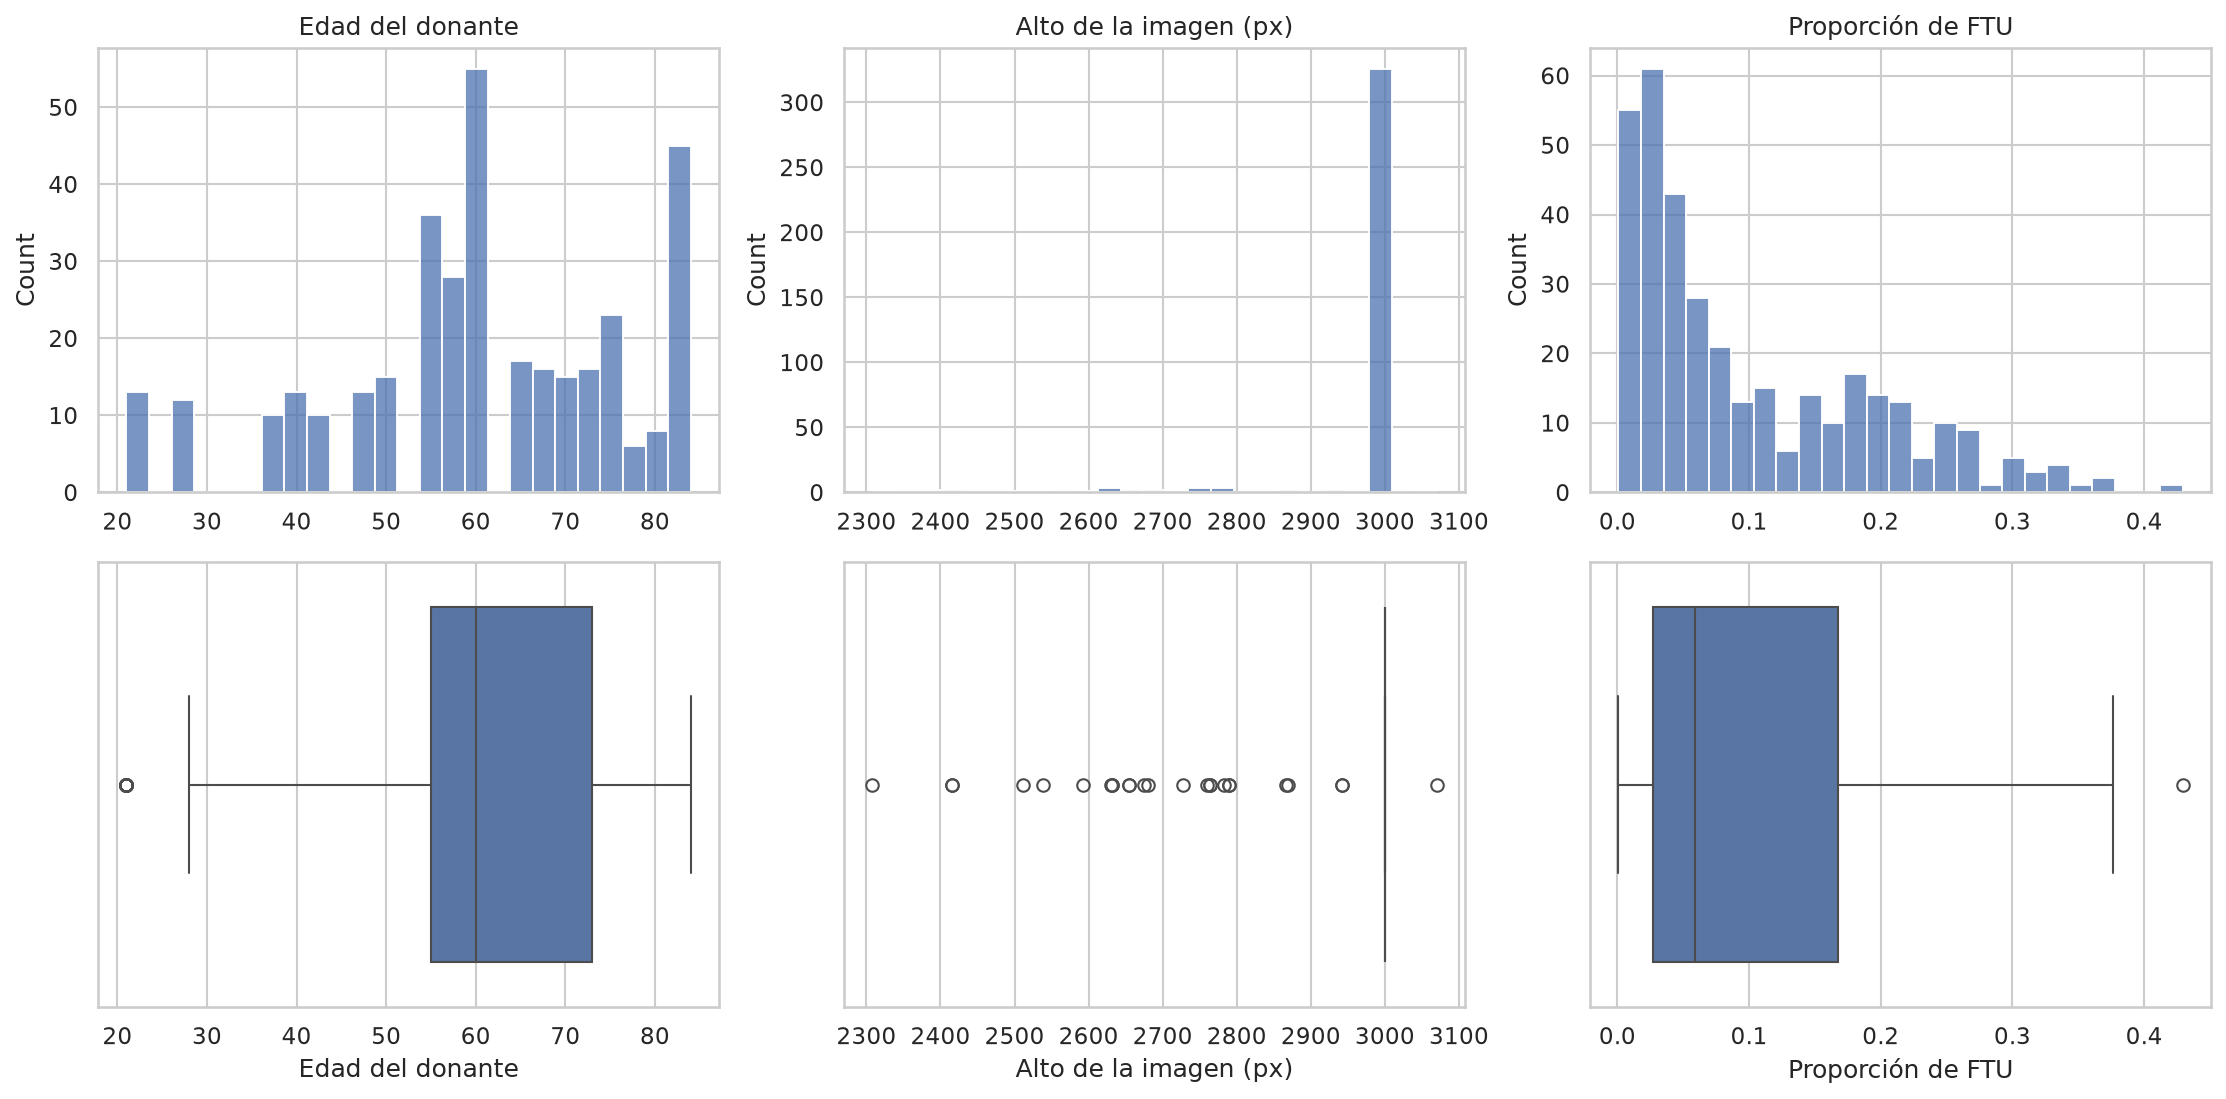
\includegraphics[width=\textwidth]{univariadas.png}
\caption{Histogramas y diagramas de caja de edad, alto de imagen y proporción de FTU.}
\end{figure}

En \texttt{age} la distribución va de 21 a 84 años, se concentra entre los 55 y los 73 y tiene una
mediana de 60 años. Es una población de donantes mayoritariamente adulta mayor, y la cola hacia los
donantes jóvenes es bastante más delgada, de modo que el conjunto no representa por igual todas las
edades.

En \texttt{img\_height} el gráfico se ve casi como una sola barra: 326 de las 351 imágenes son de
$3000 \times 3000$ píxeles y el resto son algo más pequeñas. El diagrama de caja marca todas esas
imágenes menores como outliers, pero como ya se explicó no son errores.

En \texttt{mask\_frac} la distribución está claramente sesgada a la derecha: la mediana es 0.059,
alrededor del 6\,\% de la imagen, pero existen casos que llegan a 0.43. Esto significa que en la
mayoría de las imágenes la estructura a segmentar ocupa una parte pequeña de la fotografía, lo cual
implica un problema con clases fuertemente desbalanceadas a nivel de píxel.

\subsubsection{Gráficos de barra de las variables categóricas}

\begin{figure}[H]
\centering
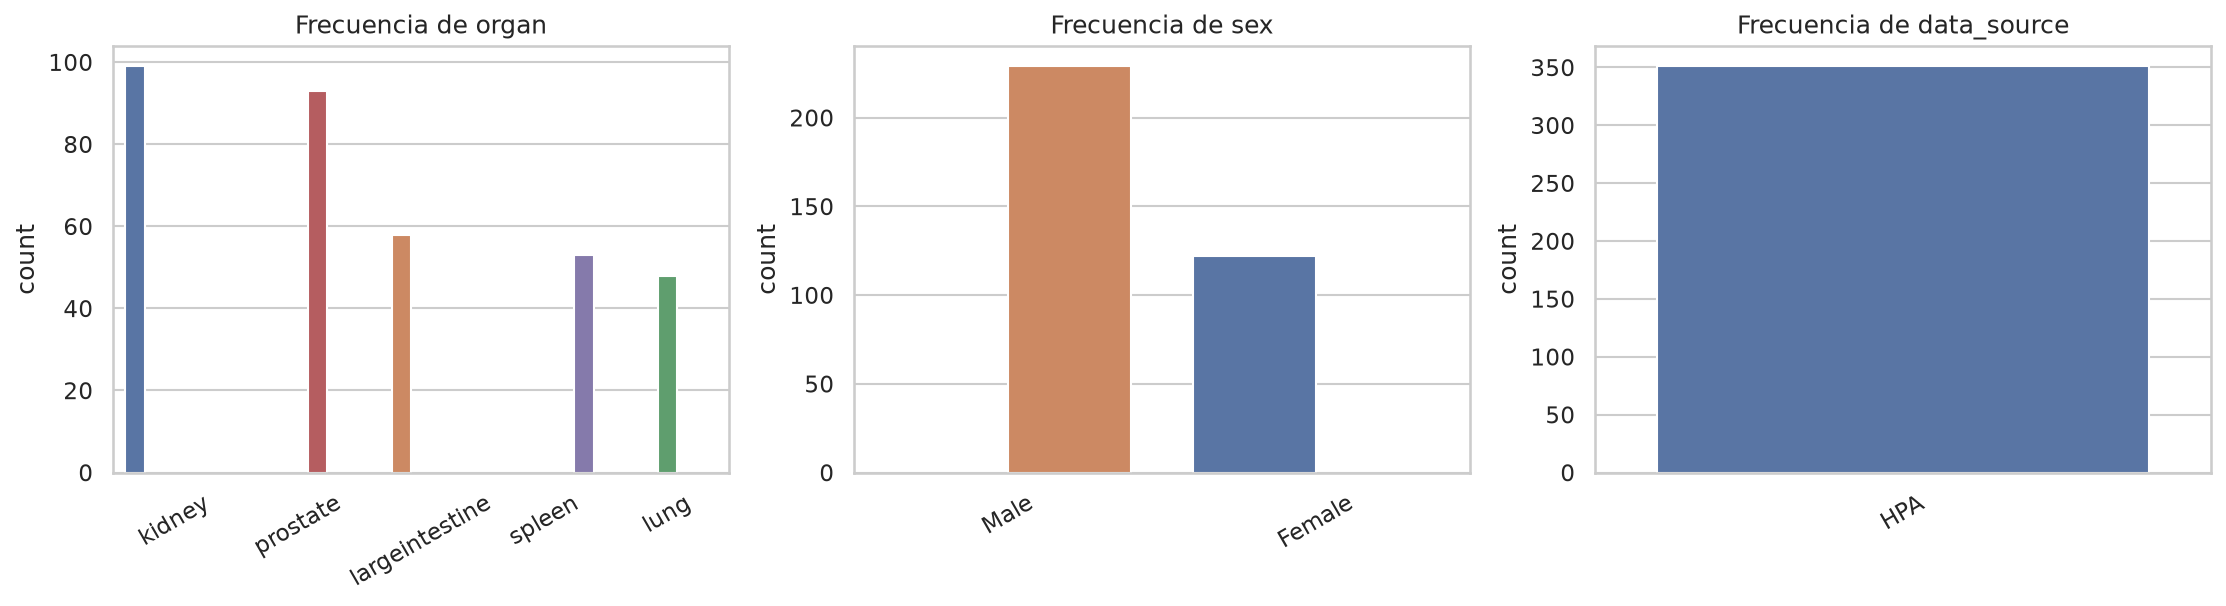
\includegraphics[width=\textwidth]{categoricas.png}
\caption{Frecuencia de órgano, sexo y fuente de datos.}
\end{figure}

Los tres gráficos de barra confirman visualmente lo descrito en las tablas de frecuencia. El caso de
\texttt{data\_source} es particularmente elocuente: una sola barra, porque las 351 filas pertenecen a
HPA. La variabilidad entre laboratorios, que constituye la dificultad principal del reto, no se puede
observar dentro de estos datos.

\subsubsection{Cruces gráficos}

\begin{figure}[H]
\centering
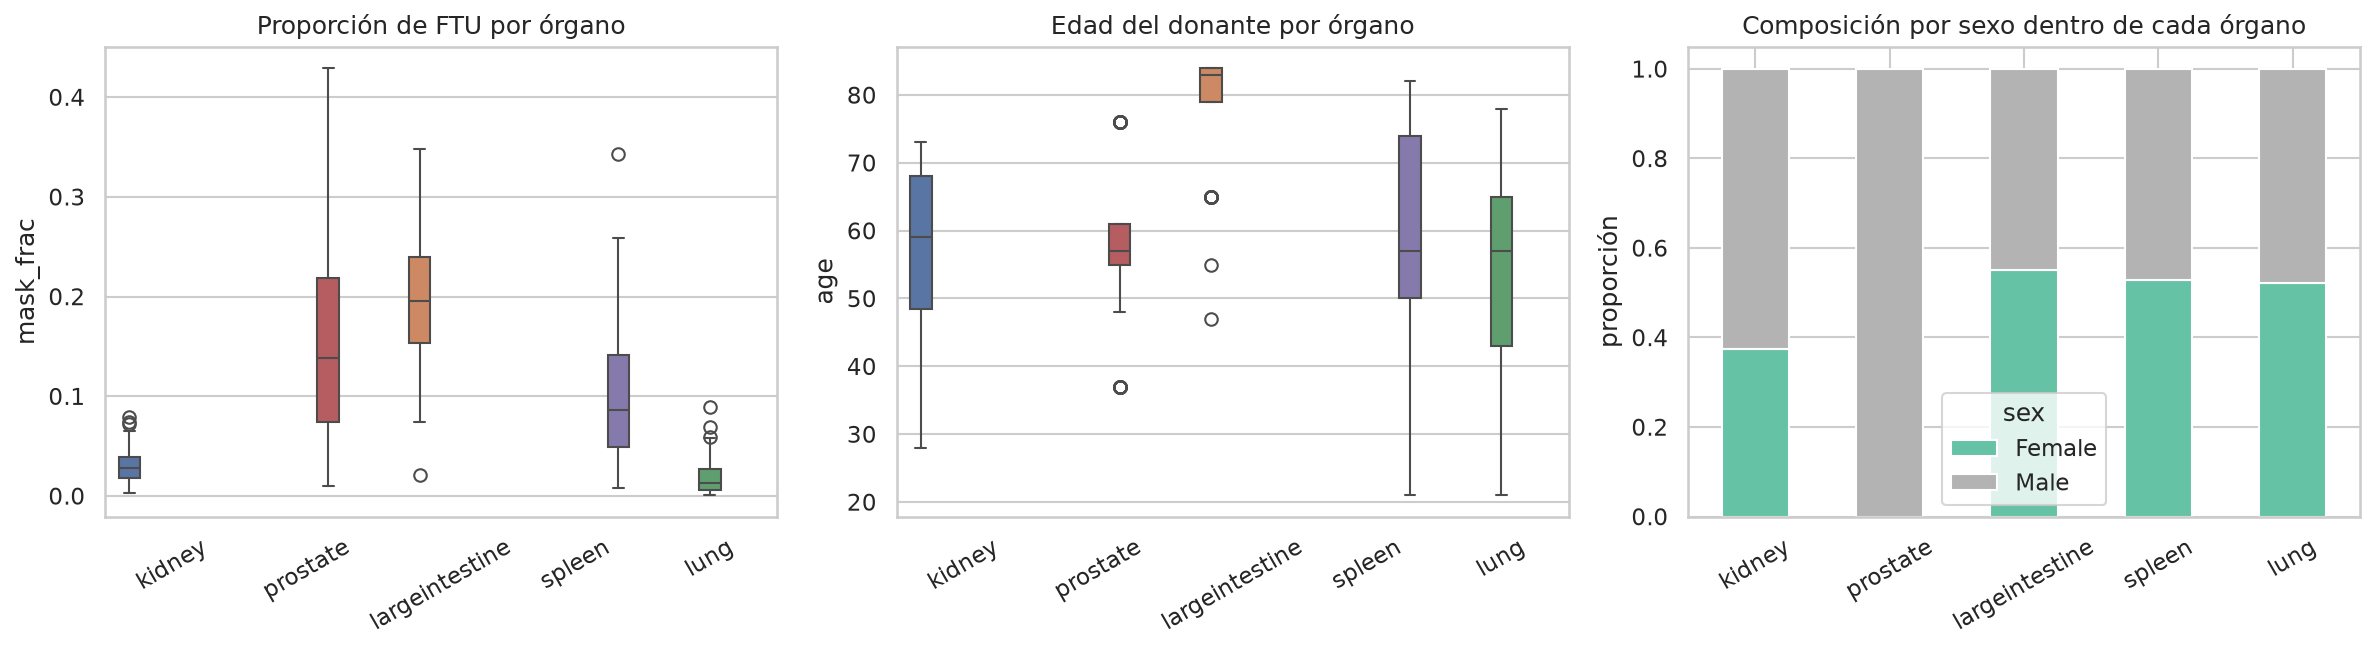
\includegraphics[width=\textwidth]{cruces.png}
\caption{Proporción de FTU por órgano, edad por órgano y composición por sexo dentro de cada órgano.}
\end{figure}

El primer panel es el más informativo. La proporción de imagen ocupada por la FTU cambia
drásticamente según el órgano: en intestino grueso la mediana es de casi 0.20 y en próstata de 0.14,
mientras que en pulmón apenas llega a 0.013 y en riñón a 0.028. Es decir, las FTU de pulmón ocupan
alrededor de quince veces menos superficie que las de intestino grueso. La dispersión también
difiere: próstata y bazo presentan cajas muy anchas y intestino grueso una más compacta. Encontrar
la FTU no es el mismo problema en cada órgano.

El segundo panel muestra el caso de intestino grueso, con mediana de 83 años frente a los 57 a 59 de
los otros cuatro órganos. El tercero muestra el caso extremo de próstata, 100\,\% masculino.

\subsubsection{Gráficos de dispersión}

\begin{figure}[H]
\centering
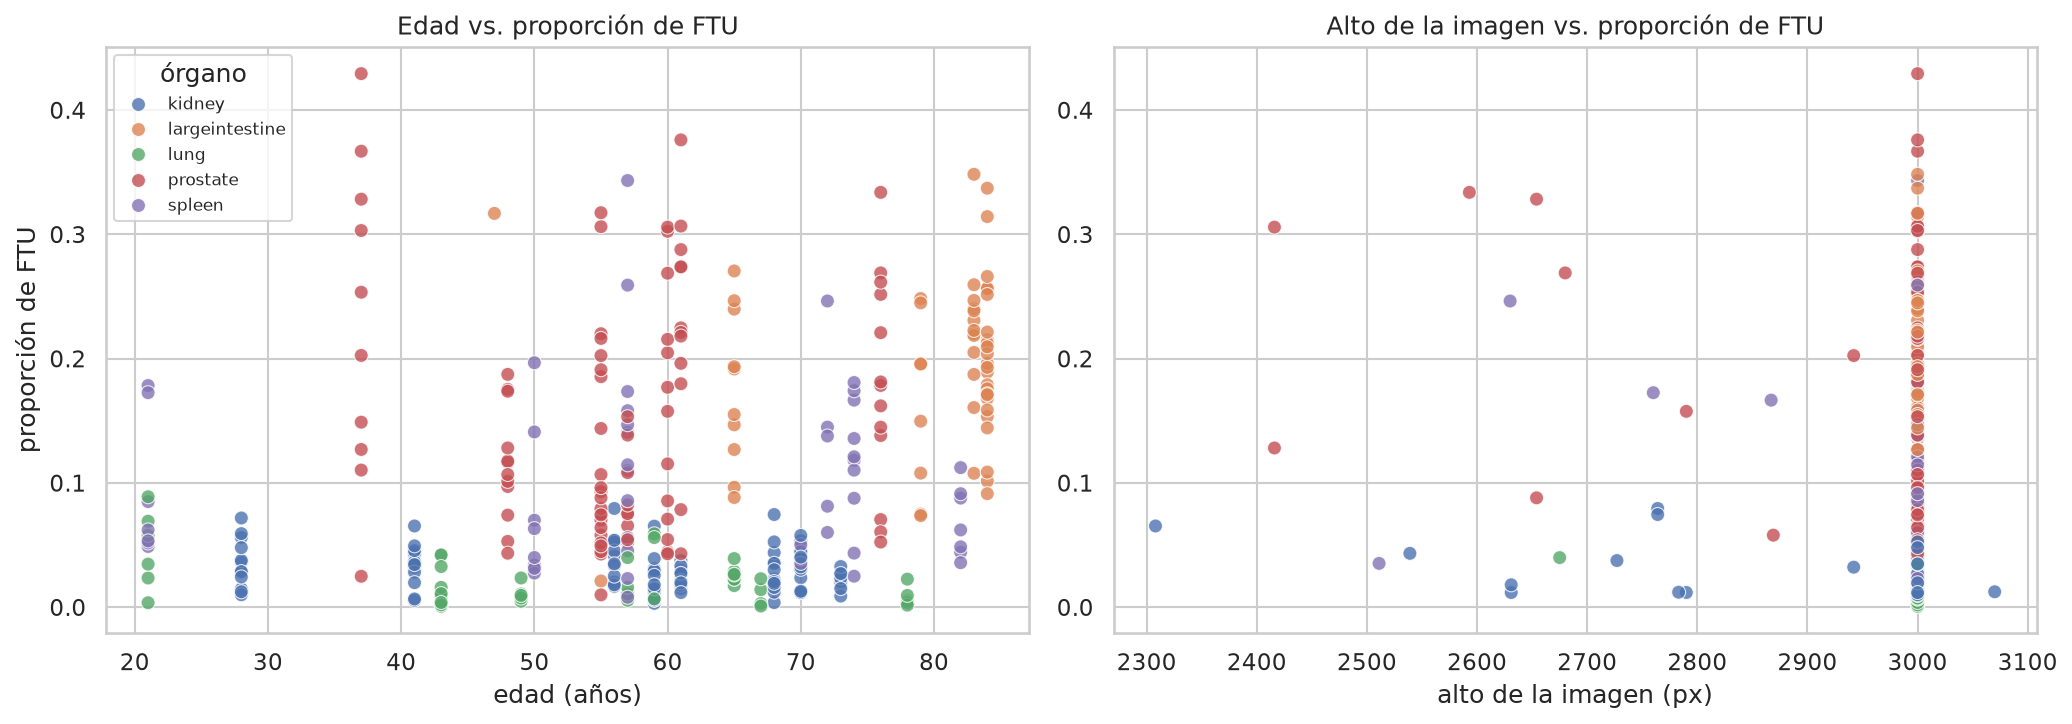
\includegraphics[width=\textwidth]{dispersion.png}
\caption{Relación entre edad y proporción de FTU, y entre tamaño de imagen y proporción de FTU,
coloreadas por órgano.}
\end{figure}

El primer gráfico de dispersión contiene el hallazgo más sutil del análisis. Si se calcula la
correlación entre edad y proporción de FTU sobre las 351 filas en conjunto, resulta $r = 0.248$: una
relación positiva débil pero visible, que invitaría a concluir que a mayor edad del donante mayor es
el tamaño de la FTU.

Al separar por órgano, esa relación desaparece o se invierte:

\begin{table}[H]
\centering
\caption{Correlación entre edad y proporción de FTU, global y por órgano}
\begin{tabular}{lrr}
\toprule
\textbf{Grupo} & \textbf{n} & \textbf{r (age, mask\_frac)} \\
\midrule
Global          & 351 & $0.248$ \\
\midrule
kidney          & 99 & $-0.178$ \\
largeintestine  & 58 & $0.139$ \\
lung            & 48 & $-0.396$ \\
prostate        & 93 & $0.003$ \\
spleen          & 53 & $0.028$ \\
\bottomrule
\end{tabular}
\end{table}

Lo que ocurre es que la correlación global no mide una relación entre edad y tamaño de FTU, sino que
captura el efecto del órgano. Intestino grueso tiene simultáneamente los donantes de mayor edad
(mediana de 83 años) y las FTU más grandes (19.6\,\% de la imagen), de modo que al mezclar todos los
órganos en una sola nube ese grupo arrastra la correlación hacia arriba. Se trata de un caso de
paradoja de Simpson: la tendencia que aparece en el agregado se contradice al observar cada
subgrupo por separado.

La conclusión práctica es doble. Primero, la edad no sirve para anticipar el tamaño de la FTU.
Segundo, y más importante, cualquier correlación calculada sobre este conjunto sin estratificar por
órgano debe mirarse con desconfianza.

El segundo gráfico confirma que los puntos se apilan casi todos sobre la línea de 3000 px, y que los
pocos que quedan a la izquierda son las imágenes recortadas. La correlación entre tamaño de imagen y
proporción de FTU es $-0.079$, prácticamente nula, lo que indica que las imágenes más pequeñas no
contienen FTU proporcionalmente más grandes ni más pequeñas. El recorte no introdujo un sesgo en la
variable objetivo.

\subsection{Exploración visual de las imágenes}

Sobre una muestra reducida de \texttt{train\_images} se decodificó la máscara completa mediante la
función inversa del rle y se superpuso sobre el tejido. Todas las muestras son cortes teñidos con
PAS, con tonos rosados y morados semejantes entre sí, y en todas hay zonas de fondo blanco donde no
hay tejido.

La máscara superpuesta muestra que las FTU no forman una sola región compacta: en la mayoría de los
órganos son varias regiones separadas dentro de la misma imagen, y su forma cambia por completo de
un órgano a otro. El contraste entre la FTU y el tejido circundante tampoco es uniforme. En intestino
grueso y próstata las estructuras se distinguen a simple vista, mientras que en pulmón y riñón la FTU
se confunde mucho más con el tejido de alrededor y ocupa una fracción mínima de la fotografía, lo
cual concuerda con lo observado en la distribución de \texttt{mask\_frac}.

%======================================================================
\section{Hallazgos y conclusiones}
%======================================================================

\subsection{Resumen de hallazgos}

\textbf{1. Variables sin información.} \texttt{pixel\_size} vale 0.4 en las 351 filas y
\texttt{tissue\_thickness} vale 4.0 en todas. Son constantes, su varianza es cero y por eso aparecen
como \texttt{NaN} en la matriz de correlación. Además \texttt{img\_height} e \texttt{img\_width} son
iguales entre sí en todas las filas y en el 93\,\% de los casos valen 3000. De las variables
tabulares, las únicas con información real son \texttt{organ}, \texttt{sex}, \texttt{age} y la
variable derivada de \texttt{rle}.

\textbf{2. Desbalance en varios ejes simultáneos.} Por órgano (99 riñones contra 48 pulmones), por
sexo (229 hombres contra 122 mujeres, en buena parte por los 93 casos de próstata) y por edad, con
una concentración fuerte entre los 55 y los 73 años. Además, órgano y edad no son independientes:
intestino grueso tiene una mediana de 83 años frente a los 57 a 59 del resto.

\textbf{3. Variable objetivo fuertemente desbalanceada.} La FTU ocupa en mediana apenas el 5.9\,\%
de la imagen, y esa proporción varía enormemente según el órgano: 19.6\,\% en intestino grueso
contra 1.3\,\% en pulmón. Un modelo de segmentación entrenado sobre estos datos enfrenta un
desbalance de clases severo a nivel de píxel, y ese desbalance no es uniforme entre órganos.

\textbf{4. Correlación global espuria.} La relación positiva entre edad y tamaño de FTU que aparece
al analizar el conjunto completo se desvanece o se invierte al estratificar por órgano. Es un caso
de paradoja de Simpson y obliga a analizar este conjunto siempre por subgrupos.

\textbf{5. La generalización no es observable.} Las 351 filas de \texttt{train.csv} tienen
\texttt{data\_source = HPA}. Las muestras de HuBMAP quedan del lado de los datos de prueba. Como la
dificultad central del reto es que el modelo funcione con muestras preparadas en laboratorios
distintos, resulta que la variabilidad que el modelo debe superar no se puede observar ni medir
dentro de los datos de entrenamiento. Este es el hallazgo de mayor peso del análisis.

\subsection{Conclusiones sobre los siguientes pasos}

\begin{enumerate}
  \item \textbf{Descartar las variables constantes.} \texttt{pixel\_size} y
        \texttt{tissue\_thickness} no aportan capacidad discriminativa y deben excluirse de
        cualquier modelo.

  \item \textbf{Tratar el problema como segmentación desbalanceada.} Con una mediana de 5.9\,\% de
        píxeles positivos, un modelo que predijera fondo en toda la imagen alcanzaría más del
        94\,\% de exactitud por píxel y sería completamente inútil. Corresponde emplear métricas
        como el coeficiente de Dice o la intersección sobre la unión, y funciones de pérdida
        pensadas para desbalance.

  \item \textbf{Validar por órgano y no solo de forma global.} El desempeño promedio esconde que
        pulmón y riñón, con FTU quince veces más pequeñas, son casos sustancialmente más difíciles.
        Una validación estratificada por órgano es indispensable.

  \item \textbf{Estratificar todo análisis estadístico por órgano.} La paradoja de Simpson
        encontrada demuestra que las correlaciones agregadas sobre este conjunto pueden llevar a
        conclusiones equivocadas.

  \item \textbf{Apoyarse en aumentación de color y tinción.} Dado que el conjunto de entrenamiento
        no contiene variabilidad entre fuentes, la vía razonable para preparar al modelo frente a
        las muestras de HuBMAP del conjunto de prueba es simularla mediante aumentación de datos
        sobre color, saturación e intensidad de tinción, además de normalización de tinción.
\end{enumerate}

%======================================================================
\section*{Repositorio}
\addcontentsline{toc}{section}{Repositorio}
%======================================================================

El código, el cuaderno de análisis y las fuentes de este informe están versionados en:

\begin{center}
\url{https://github.com/AleWWH1104/proyecto2-data}
\end{center}

\end{document}
